
\chapter{Model systemu rekomendacyjnego chroniącego prywatność}

W rozdziale zaproponowanie rozwiązania zwiększającego bezpieczeństwo oraz zachowanie prywatnych danych użytkownika. W tym celu wykorzystano \textit{Federated learning} omówiony w rozdziale \ref{section:federatedLearning} wraz z dodatkowymi zabezpieczeniami mającymi na celu zniwelować przedstawione problemy związane z tym rozwiązaniem. Także przedstawiono jak mógłby wyglądać proces przygotowania takiej metody dla nowo-powstałego systemu jak i dla już zaimplementowanego systemu z wykorzystaniem dostępnych bibliotek i technologii.

\section{Projekt rozwiązania}

W proponowanym rozwiązaniu (przedstawionym na rys. \ref{fig:schemat} wyróżniono trzech aktorów. Pierwszy z nich, zwykły użytkownik uczestniczy w normalnym przebiegu zaproponowanym w rozwiązaniu \textit{Federated learning}. Użytkownik na podstawie swoich danych poprawia otrzymany przez serwer model, następnie bez ujawniania swoich danych przekazuje dalej wyłącznie poprawiony przez siebie model.

Jednym z potencjalnych problemów może być założenie, że użytkownicy będą uczciwie uczestniczyć w całym omawianym procesie. Oznacza, to że użytkownik może zmniejszyć skuteczność modelu rekomendacji poprzez umieszczenie w nich niepoprawnych danych (niezgodnych z rzeczywistością). W przypadku pojedynczego użytkownika, który próbuje zakłócić pracę systemu istnieje mechanizm uśredniający otrzymane wyniki od wszystkich użytkowników. Jednak w przypadku zorganizowanego ataku z wielu kont wyłącznie normalizacja może nie być wystarczająca. W celu poradzenia sobie z tym problemem wprowadzono drugi typ aktora - użytkownik niezaufany, który ma możliwość wyłącznie otrzymania modelu od serwera głównego. Jest on wyłączony z usprawnienia udostępnianego modelu (nie wysyła on swoich rezultatów uczenia). Tego typu użytkownik po określonym czasie użytkowania systemu, ilości wystawionych ocen lub po odpowiednim procesie weryfikacyjnym może zostać przemianowany na zwykłego użytkownika uczestniczącego w procesie usprawniania wspólnego modelu.

Kolejnym problemem może być koszt nauki na systemach mobilnych. Niektórzy użytkownicy mogą posiadać słabszy sprzęt (zasoby sprzętowe czy bateria), który może uniemożliwić ponowne uczenie otrzymanego modelu na urządzeniu. W przypadku wolnego łącza lub jego braku, problemem może być pobieranie lub odesłanie modelu do głównego serwera. W tym celu użytkownik z ograniczonymi zasobami zostałby zmuszony do przesłania swoich zaszyfrowanych danych do serwera, tam wykorzystując właściwości szyfrowania homomorficznego model zostałby zaktualizowany, a rekomendacje przesłane do użytkownika.

\begin{figure}[h]
    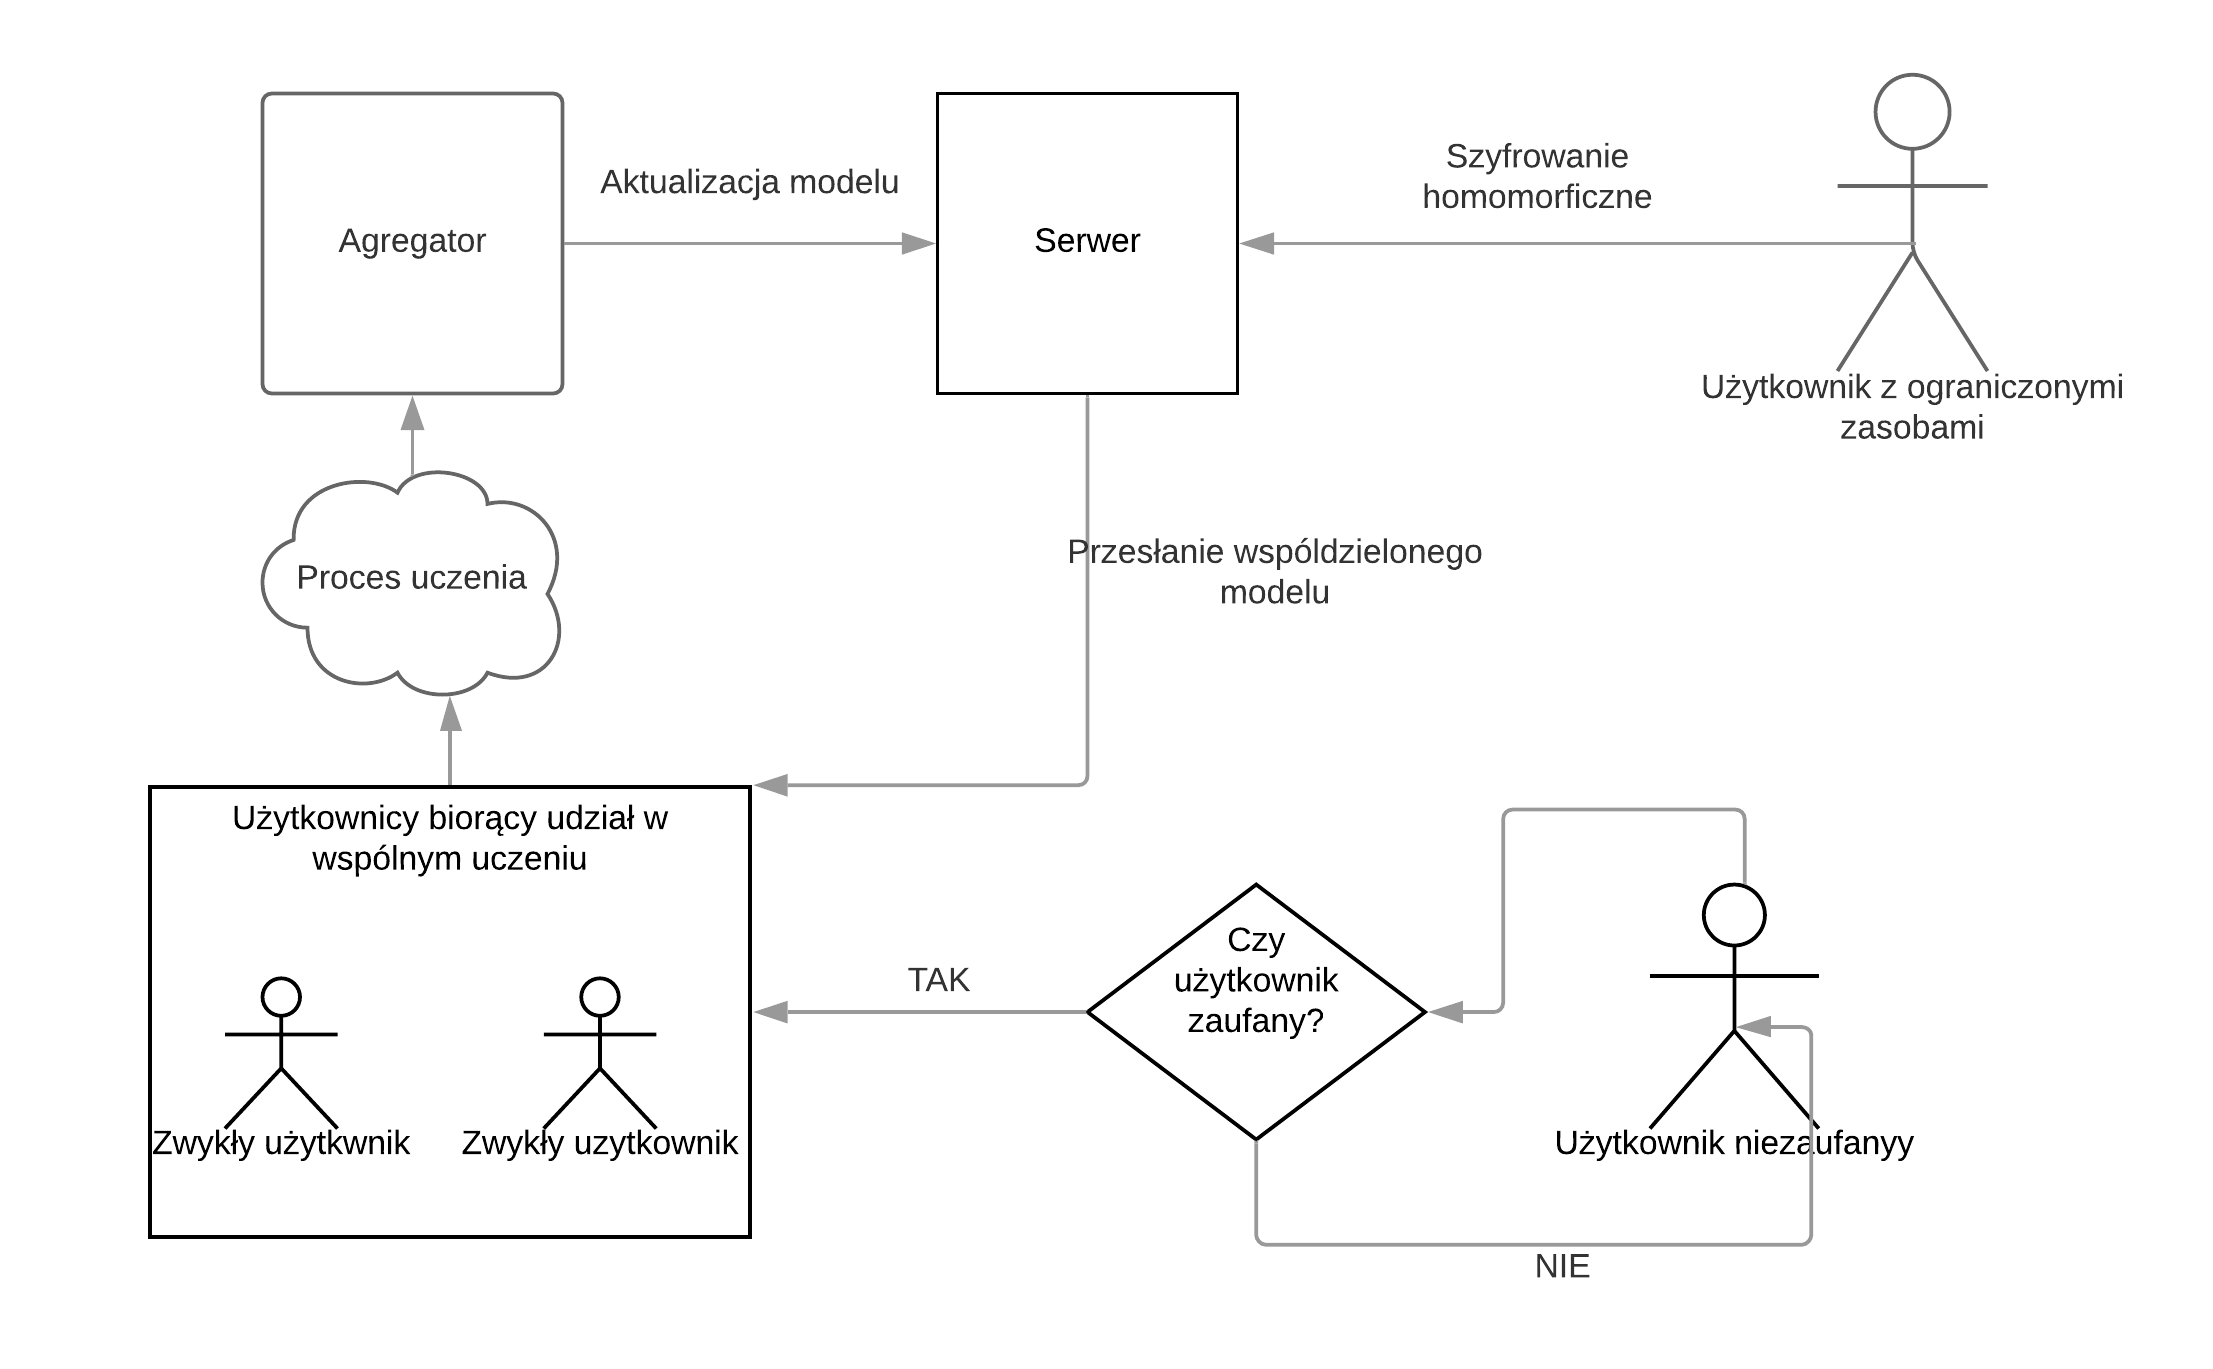
\includegraphics[scale=0.75]{schemat_protokolu.png}
    \caption{Schemat bezpiecznego protokołu.}
    \label{fig:schemat}
\end{figure}

\section{Fazy budowania systemu rekomendacyjnego}

Podczas implementacji systemu rekomendacyjnego wykorzystano typowy przepływ (przedstawiony na rysunku \ref{fig:rs_pipeline}) używany do tworzenia tego typu serwisów, który składa się z następujących pięciu faz \cite{rs_in_real}:
\begin{itemize}
    \item wstępne przetwarzanie - na ten etap składają się czynności związane z transformacją danych do macierzy użytkownik-produkt oraz normalizacja w celu spłaszczenia wartości odstających (użytkownicy, którzy są nad wyraz pozytywni oraz negatywni w stosunku do dawania ocen),
    \item trenowanie - proces budowania modelu,
    \item optymalizacja hiper parametrów - wielokrotne trenowanie w celu dostrojenia parametrów w taki sposób, aby uzyskać jak najlepsze wyniki,
    \item przetwarzanie końcowe - sortowanie danych w celu uzyskania N najlepszych rekomendacji dla użytkownika, filtrowanie oraz wykluczenie wcześniej zakupionych lub negatywnie ocenionych przedmiotów,
    \item ewaluacja - testowanie stworzonego modelu poprzez ukrywanie/maskowanie ocen, a następnie użycie miar do ewaluacji (szczegółowo opisane w podrozdziale \ref{metryki}).
\end{itemize}{}

\begin{figure}[h]
    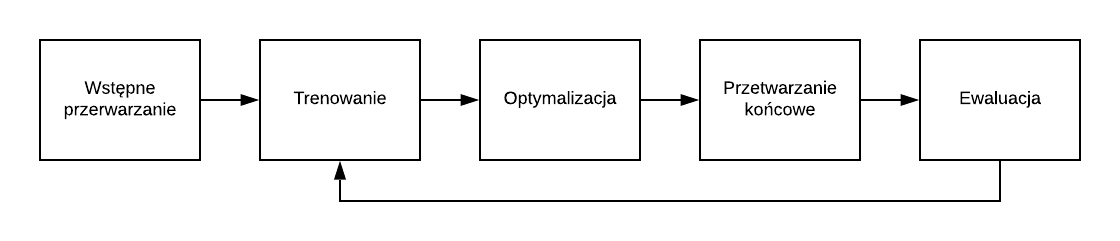
\includegraphics[scale=0.85]{rs_pipeline.png}
    \caption{Fazy przepływu podczas tworzenia systemu rekomendacyjnego.}
    \label{fig:rs_pipeline}
\end{figure}

\section{Dane testowe}\label{dane}

Do testów wykorzystano zbiór MovieLens (dostępny na stronie \url{https://grouplens.org/datasets/movielens}) zebrany przez laboratorium badawcze \textit{GroupLens} działające na Wydziale Informatyki i Inżynierii Uniwersytetu w Minnesota. Dane zawierają zanonimizowane informacje o filmach (nazwa, tagi) oraz użytkownikach. Oceny filmów zaprezentowane są w skali pięciostopniowej z przyrostem o pół oceny (od 0.5 do 5.0). Fragment danych został przedstawiony na rys. \ref{fig:movie_lens} w formie macierzy film-użytkownik (kolumny zawierają identyfikator filmu, natomiast wiersze identyfikator użytkownika).

\begin{figure}[h]
    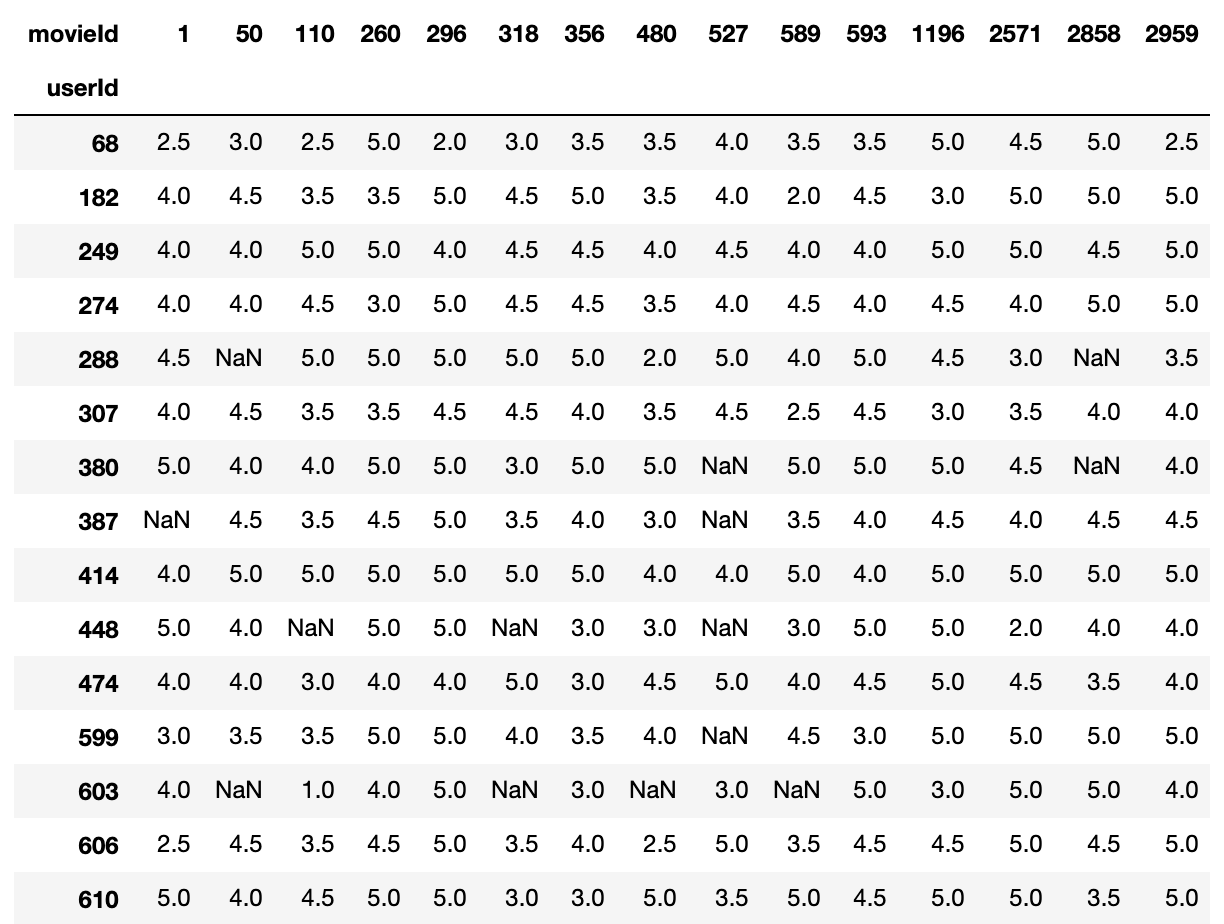
\includegraphics[scale=0.6]{movie_lens.png}
    \caption{Przykładowe dane zawarte w zbiorze \textit{MovieLens}.}
    \label{fig:movie_lens}
\end{figure}

\section{Przegląd dostępnych technologii}\label{technologie}

Istnieje wiele dostępnych bibliotek czy frameworków umożliwiających na implementacje rozwiązań typu \textit{Federated learning}. Większość z nich umożliwia na napisanie kodu w języku Python. Jednymi z bardziej popularnych oraz dobrze udokumentowanych są następujące technologie:

\begin{itemize}
    \item PySyft - narzędzie opracowane przez grupę OpenMinded. PySyft rozszerza popularne biblioteki takie jak: PyTorch, Tensorflow oraz Keras o możliwość zdalnego wykonywania, szyfrowania homomorficznego czy obliczenia z wykorzystaniem wielu użytkowników (\url{https://github.com/OpenMined/PySyft}),
    \item Tensorflow Federated - biblioteka wykorzystywana do uczenia maszynowego i innych obliczeń na danych niescentralizowanych oparta o otwarty kod źródłowy. Stworzona w celu badań oraz eksperymentowania z koncepcją \textit{Federated learning} (\url{https://github.com/tensorflow/federated}),
    \item FATE - pozwala na implementację protokołów bezpiecznego obliczania opartych o szyfrowanie homomorficzne oraz obliczanie wieloczęściowe. Wspiera wiele algorytmów uczenia maszynowego: regresję logistyczną, algorytmy oparte o drzewa czy uczenie głębokie (\url{https://github.com/FederatedAI/FATE}), 
    \item Baidu PaddleFL - biblioteka o otwartym kodzie źródłowym, umożliwiająca na łatwe wdrożenie podejścia \textit{Federated learning} na dużą skalę z wykorzystaniem rozproszonych klastrów, (\url{https://github.com/PaddlePaddle/PaddleFL}),
    \item NVIDIA Clara - biblioteka stosowana w przetwarzaniu obrazów medycznych, genomice czy "smart szpitalach", wykorzystująca wspólne uczenie w budowaniu modeli (\url{https://developer.nvidia.com/clara}).
\end{itemize}

\section{Fragmenty implementacji}

Na listingu \ref{lst:initPyTorch} pokazano jak inicjowani są klienci uczestniczący w procesie uczenia oraz rozdzielenie danych na poszczególnych klientów z wykorzystaniem bibilioteki \textit{PySyft}. Klienci tworzeni są poprzez wywołanie konstruktora \textit{VirtualWorker}, natomiast za pomocą metody \textit{federate} rozdzielane są dane dla klientów 1 oraz 2, które trafiają do dostawcy (\textit{FederatedDataLoader}).

\begin{lstlisting}[language=Python, caption={Inicjalizacja klientów oraz podział danych}, label={lst:initPyTorch}, captionpos=b]
hook = sy.TorchHook(torch)
client1 = sy.VirtualWorker(hook, id="client1")
client2 = sy.VirtualWorker(hook, id="client2")

train_set = UserItemRatingDataset(X_train, y_train)
test_set = UserItemRatingDataset(X_test, y_test)

federated_train_loader = sy.FederatedDataLoader(
    train_set.federate((client1, client2)), 
    batch_size=64, shuffle=True)

test_loader = torch.utils.data.DataLoader(
    test_set, batch_size=64, shuffle=True)
\end{lstlisting}

Kolejny fragment kodu (listing \ref{lst:initTFFederated}) pokazuje tworzenie procesu uczenia oparte o wielu klientów przy pomocy biblioteki \textit{Tensorflow Federated}. Odbywa się to za pomocą funkcji \textit{build\_federated\_averaging\_process}, która przyjmuje dwa parametry:
\begin{itemize}
    \item \textit{model\_fn} - funkcja tworząca model,
    \item \textit{client\_optimizer\_fn} - funkcja służąca do optymalizacji wyników klientów.
\end{itemize}

Podczas tworzenia modelu wykorzystano podbibliotekę \textit{Keras} do stworzenia modelu (\textit{create\_keras\_model}). Następnie wykorzystano metodę umożliwiającą na stworzenie współdzielonego modelu wykorzystując wynik otrzymany z poprzedniego kroku (metoda \textit{from\_keras\_model)}.

\begin{lstlisting}[language=Python, caption={Tworzenie "trenera" - Tensorflow Federated}, label={lst:initTFFederated}, captionpos=b]
federated_train_data = make_federated_data(train_dataset, 
train_dataset.client_ids)

def model_fn():
    rn_model = create_keras_model()

    return tff.learning.from_keras_model(
      keras_model=rn_model,
      input_spec=preprocessed_sample_dataset.element_spec,
      loss=tf.keras.losses.MeanSquaredError(),
      metrics=[tf.keras.metrics.SparseCategoricalAccuracy()])

trainer = tff.learning.build_federated_averaging_process(
  model_fn=model_fn,
  client_optimizer_fn=lambda: SGD(lr=0.001))
state = trainer.initialize()
\end{lstlisting}

Tak utworzony proces może zostać zainicjowany oraz wykorzystany do nauki na danych.

\section{Eksperymenty}

W sekcji zaprezentowano założenia eksperymentów z bibliotekami (omówione w podrozdziale \ref{technologie}) związanymi z pojęciem \textit{Federated Learning} oraz uzyskane wyniki. Eksperymenty mają na celu sprawdzenia łatwości implementacji, porównania czasu nauki oraz uzyskane wyniki w zależności od liczby klientów biorących udział w procesie nauki.

Założenia/ograniczenia przeprowadzanego eksperymentu:
\begin{itemize}
    \item dane testowe: \textit{MovieLens} (szerzej omówione i zaprezentowane w podrozdziale \ref{dane}),
    \item liczba epok (pojedyncza modyfikacja wag): 4,
    \item liczba klientów: od 1 do 10 klientów,
    \item wykorzystane biblioteki: \textit{PySyft} oraz \textit{TensorflowFederated}.
\end{itemize}

Środowisko testowe:
\begin{itemize}
    \item procesor: 2,3 GHz Dual-Core Intel Core i5,
    \item pamięć: 16 GB 2133 MHz LPDDR3,
    \item język programowania: Python 3.8,
    \item środowisko programistyczne: PyCharm CE 2020.02.
\end{itemize}

\begin{figure}[h]
    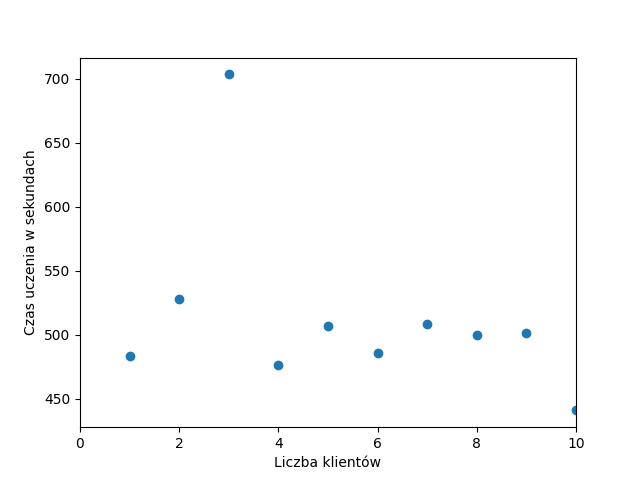
\includegraphics[scale=0.7]{learning_time.png}
    \caption{Czas uczenia w zależności od liczby klientów (\textit{PySyft)}.}
    \label{fig:learning_time}
\end{figure}

Rysunek \ref{fig:learning_time} przedstawia czas nauki dla każdej testowanej liczby klientów. Jak widać czas nauki w zależności od liczby klientów nie rośnie, lecz utrzymuje stały, równy poziom (od 470 do 525 sekund). Jedynie dla trzech klientów czas stosunkowo odbiega od pozostałych wyników (czas uczenia wyniósł 700 sekund). Może to być spowodowane chwilowym spadkiem wydajności komputera na którym przeprowadzano testy.

\begin{figure}[h]
    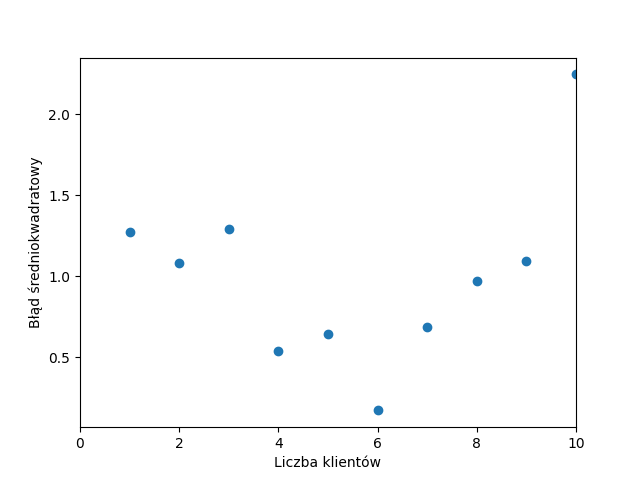
\includegraphics[scale=0.7]{loss_result.png}
    \caption{Średni błąd kwadratowy w zależności od liczby klientów (\textit{PySyft}).}
    \label{fig:loss_result}
\end{figure}

Na kolejnym rysunku (\ref{fig:loss_result}) pokazano jaka jest wartość błędu w zależności od liczby klientów. Uzyskane dane wskazują na to, że większa liczba klientów biorących udział w uczeniu nie wpływa na miarę błędu (uzyskane wartości są w przedziale od 0.2 do 1.25). W niektórych przypadkach wyższy wskaźnik błędu może być spowodowany drobnymi pomyłkami w implementacji używanego modelu.

Niestety w przypadku modelu zaimplementowanego z użyciem \textit{Tensorflow} oraz \textit{Keras} nie udało się zmodyfikować w taki sposób, aby wykorzystać podejście \textit{Federated learning} z wykorzystaniem narzędzia \textit{Tensorflow Federated}. Jest to spowodowane faktem, że w przeciwieństwie do \textit{PySyft} wymaga użycia dedykowanej struktury wspieranej wyłącznie przez \textit{Tensorflow Federated}. Problem objawiał się w postaci błędnej liczby wejść do otrzymanych danych. Mała liczba przykładów znajdujących się w dokumentacji sprawiła, że proces implementacji był skomplikowany oraz wymagało to zapoznanie się z kodem źródłowym biblioteki.
